\documentclass[tikz,border=8pt]{standalone}
% Shared look for every TikZ diagram. Load with \input{../../tools/tikz-style.tex}
\usepackage[T1]{fontenc}
\usepackage{lmodern}
\renewcommand{\sfdefault}{lmr}  % diagrams use the same serif as the text
\usetikzlibrary{arrows.meta, positioning, shapes.geometric, calc, fit, backgrounds}
\definecolor{cblue}{HTML}{4C78A8}
\definecolor{corange}{HTML}{F58518}
\definecolor{cgreen}{HTML}{54A24B}
\definecolor{cred}{HTML}{E45756}
\definecolor{cpurple}{HTML}{B279A2}
\definecolor{cgrey}{HTML}{6B6B6B}
\tikzset{
  every picture/.style={font=\sffamily, line width=1.2pt},
  box/.style={draw=#1, fill=#1!12, rounded corners=4pt, align=center, inner sep=7pt, minimum height=1.1cm},
  box/.default=cgrey,
  arrow/.style={-{Stealth[length=3mm]}, draw=cgrey, line width=1.4pt},
  title/.style={font=\sffamily\bfseries\Large},
  note/.style={font=\sffamily\small, text=cgrey, align=center},
}
\AtBeginDocument{\hyphenpenalty=10000 \exhyphenpenalty=10000}

\begin{document}
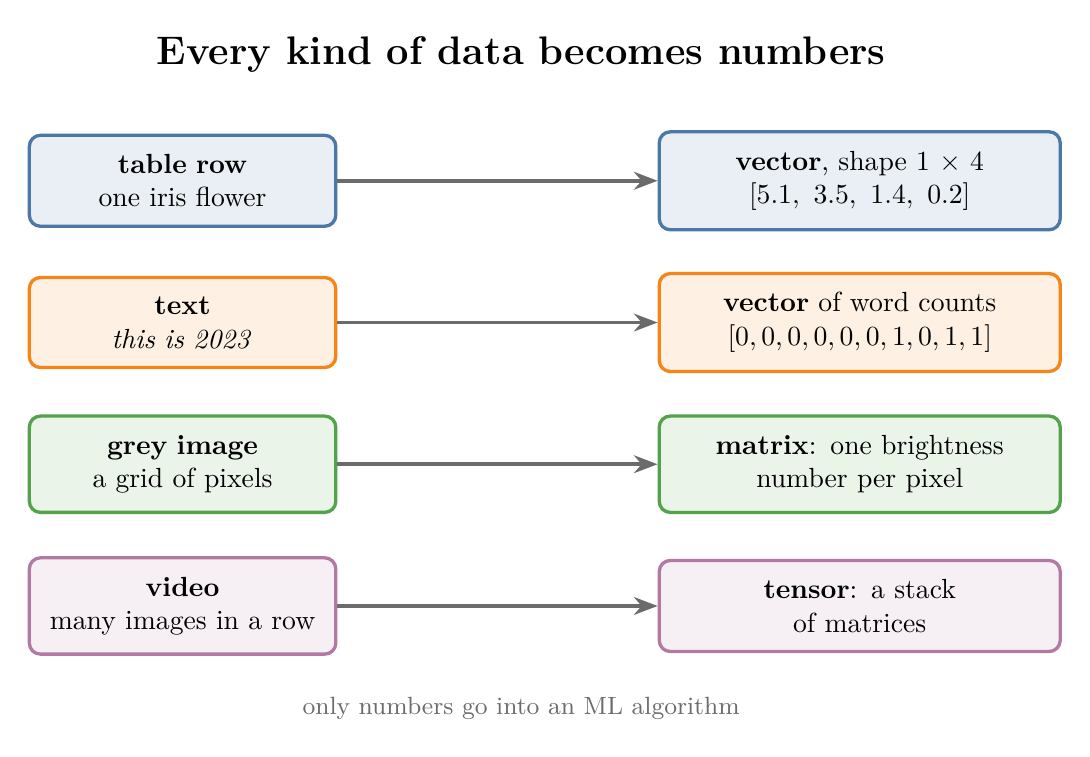
\begin{tikzpicture}
  \node[title] at (4.3,4.2) {Every kind of data becomes numbers};
  % table row -> vector
  \node[box=cblue, text width=3.4cm] (t) at (0,2.6) {\textbf{table row}\\ one iris flower};
  \node[box=cblue, text width=4.6cm] (tv) at (8.6,2.6) {\textbf{vector}, shape $1\times 4$\\ $[5.1,\ 3.5,\ 1.4,\ 0.2]$};
  \draw[arrow] (t) -- (tv);
  % text -> vector
  \node[box=corange, text width=3.4cm] (x) at (0,0.8) {\textbf{text}\\ \textit{this is 2023}};
  \node[box=corange, text width=4.6cm] (xv) at (8.6,0.8) {\textbf{vector} of word counts\\ $[0,0,0,0,0,0,1,0,1,1]$};
  \draw[arrow] (x) -- (xv);
  % image -> matrix
  \node[box=cgreen, text width=3.4cm] (i) at (0,-1.0) {\textbf{grey image}\\ a grid of pixels};
  \node[box=cgreen, text width=4.6cm] (iv) at (8.6,-1.0) {\textbf{matrix}: one brightness\\ number per pixel};
  \draw[arrow] (i) -- (iv);
  % video -> tensor
  \node[box=cpurple, text width=3.4cm] (v) at (0,-2.8) {\textbf{video}\\ many images in a row};
  \node[box=cpurple, text width=4.6cm] (vv) at (8.6,-2.8) {\textbf{tensor}: a stack\\ of matrices};
  \draw[arrow] (v) -- (vv);
  \node[note] at (4.3,-4.1) {only numbers go into an ML algorithm};
\end{tikzpicture}
\end{document}
